\documentclass[english,serif,mathserif,xcolor=pdftex,dvipsnames,table]{beamer}

\usepackage[T1]{fontenc}
\usepackage[utf8]{inputenc}

\usetheme[informal]{s3it}
\usepackage{s3it}

\title[Introduction to Python]{%
  A Short and Incomplete Introduction to Python
}
\subtitle{\bfseries Part 11: Ending remarks}
\author[R.~Murri]{%
  \textbf{Riccardo Murri} \texttt{<riccardo.murri@uzh.ch>}, \\
  Sergio Maffioletti \texttt{<sergio.maffioletti@uzh.ch>}
  \\
  S3IT: Services and Support for Science IT,
  \\
  University of Zurich
}
\date{January 23, 2018}


\begin{document}

% title frame
\maketitle



\begin{frame}
  \frametitle{There is more to Python than this\ldots}

  The time and scope of this course is quite limited.

  \+
  Here is an (incomplete) list of Python features that you might
  want to look up as you become more experienced in the language:
  % FIXME: mettere un link per ciascuna di queste!
  \begin{itemize}
  \item \href{https://github.com/gc3-uzh-ch/python-course}{Object-oriented programming}
  \item
    %\href{http://docs.python.org/2/tutorial/classes.html\#generators}{Generators}
    %and
    \href{http://docs.python.org/2/tutorial/classes.html\#iterators}{Iterators}
  \item
    \href{http://www.artima.com/weblogs/viewpost.jsp?thread=240808}{Decorators}
  \item Class-level attributes, \href{http://stackoverflow.com/a/12179752/1808780}{classmethods, staticmethods}
  \item Properties and accessors
  \item \href{http://stackoverflow.com/a/6581949/459543}{Metaclasses}
  \end{itemize}
\end{frame}


\begin{frame}
  \frametitle{Other useful libraries}

  \begin{describe}{SciPy, \url{https://docs.scipy.org/doc/scipy/reference/}}
    A library of commonly used features in numerical programming (FFT,
    optimization, special functions, statistics, linear algebra, etc.)
  \end{describe}

  \begin{describe}{skimage, \url{https://scikit-image.org/}}
    A collection of algorithms for image processing.
  \end{describe}
\end{frame}


\begin{frame}
  \frametitle{Other useful libraries}

  \begin{describe}{PyTorch, \url{https://pytorch.org/}}
    Deep Learning Framework
  \end{describe}

  \begin{describe}{sklearn, \url{https://scikit-learn.org}}
    Machine Learning in Python
  \end{describe}

  \begin{describe}{spaCy, \url{https://spacy.io/}}
    Natural Language Processing in Python
  \end{describe}
\end{frame}


\begin{frame}
  \frametitle{Other useful libraries: interactivity}

  \begin{describe}{Plotly, \url{https://plot.ly/python/}}
    Create interactive graphs and charts.
  \end{describe}

  \begin{describe}{Dash, \url{https://plot.ly/products/dash/}}
    A Python framework for building analytics web applications
    entirely in Python.
  \end{describe}

\end{frame}


\begin{frame}
  \frametitle{Other useful libraries: performance}

  \begin{describe}{Dask, \url{http://docs.dask.org/en/latest/why.html}}
    Transparently distribute NumPy and PanDas computations across
    multiple cores or even a batch-computing cluster.
  \end{describe}

  \begin{describe}{Numba, \url{http://numba.pydata.org/}}
    A compiler to accelerate Python+NumPy functions.
  \end{describe}

\end{frame}


\begin{frame}[fragile]
  \frametitle{Want even more? Look into PyPI}
  \small

  \href{http://pypi.python.org}{PyPI} is \emph{the} index of Python
  software packages.  It currently indexes 165'633 packages, so the
  choice is really vast.

  \begin{center}
    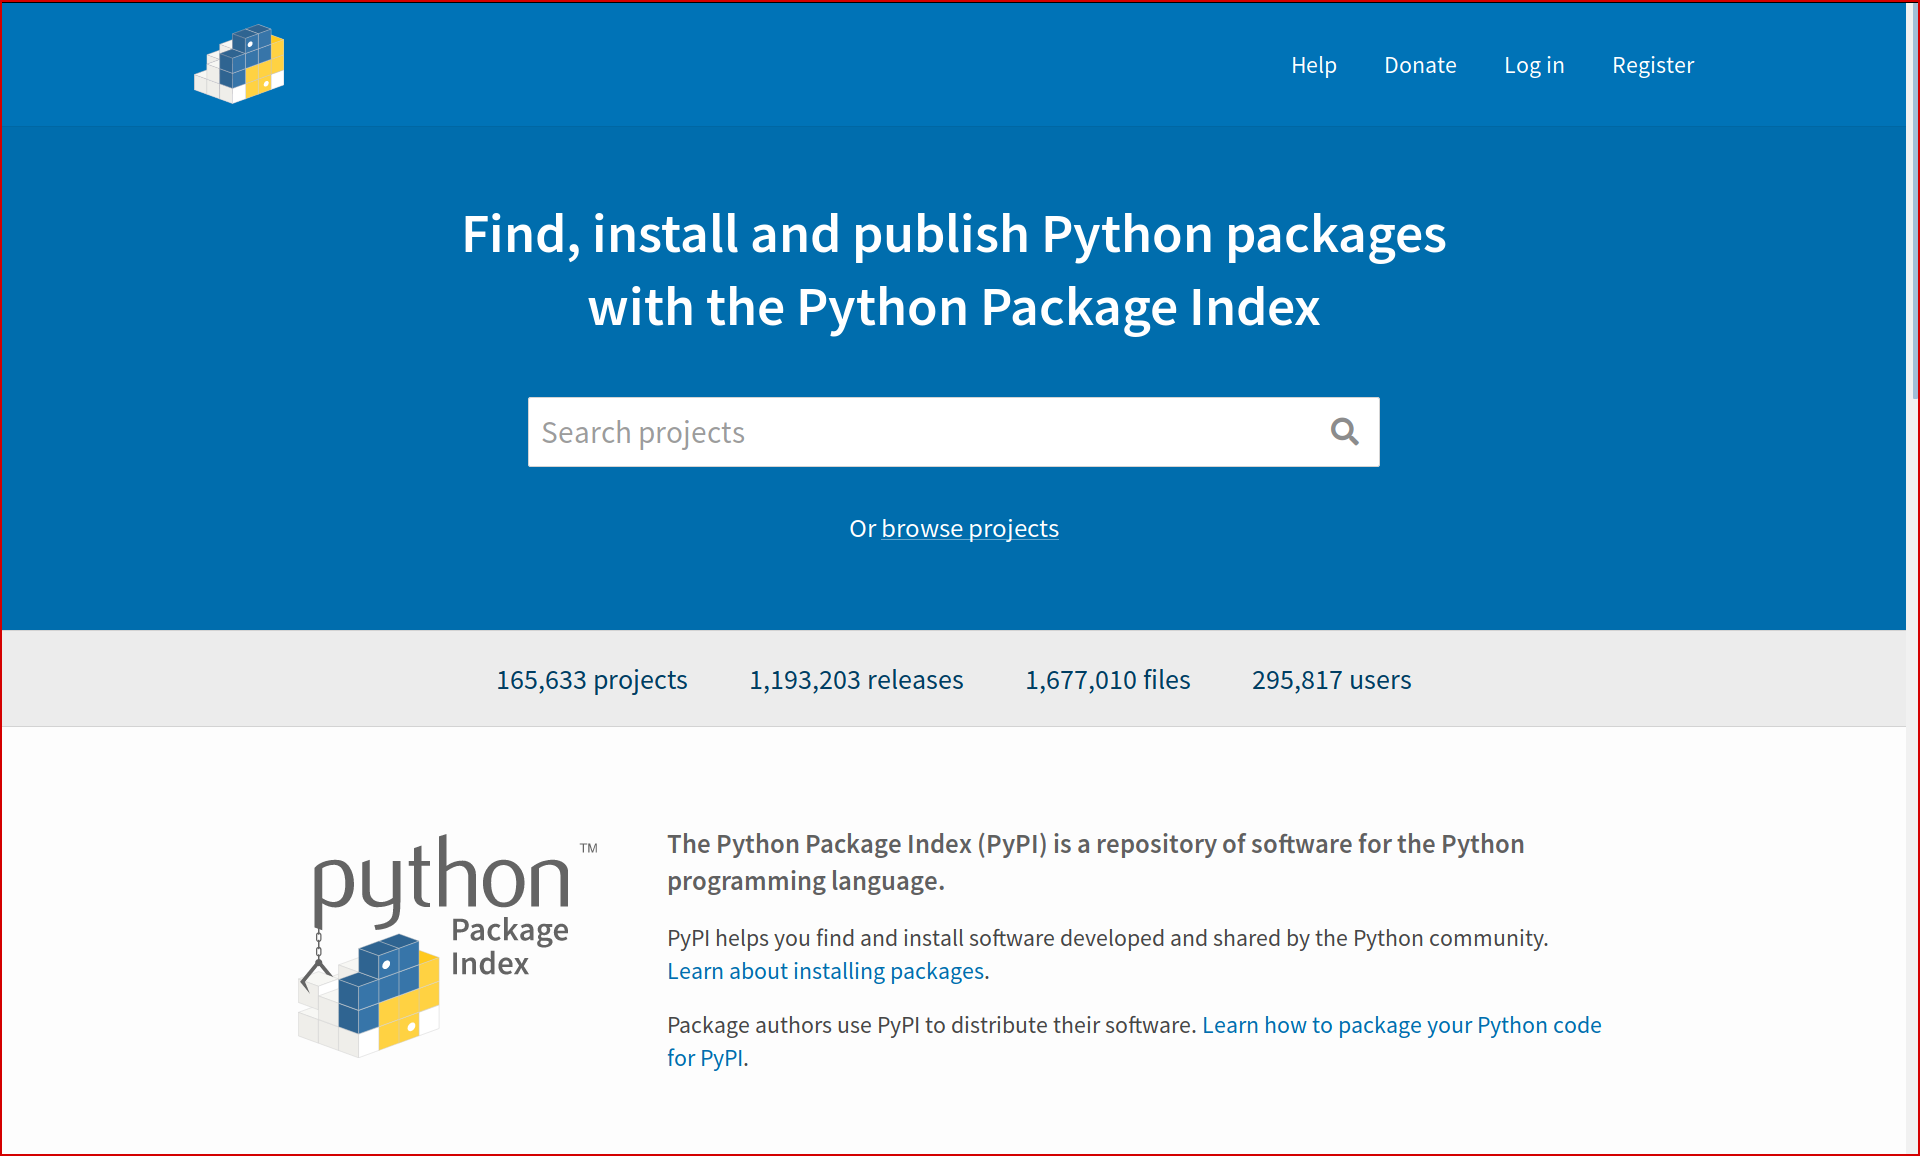
\includegraphics[width=0.60\textwidth]{fig/pypi_screenshot.png}
  \end{center}

  Almost all packages can be installed with a single command by
  running:
\begin{semiverbatim}
             \href{https://pypi.python.org/pypi/pip}{\texttt{pip install \emph{packagename}}}
\end{semiverbatim}

\end{frame}


\begin{frame}[fragile]
  \frametitle{Where to go now?}

  \begin{itemize}
    \item \textbf{The Python tutorial},
      {\small \url{http://docs.python.org/tutorial/}}
    \item {Dive into Python 3}
      {\small \url{https://www.cmi.ac.in/~madhavan/courses/prog2-2012/docs/diveintopython3/index.html}}
  %   \item {The Zen of Python in 3 days},
  %     {\small \url{http://pixelmonkey.org/pub/python-training/}}
    \item {The DataCamp courses (videos)}
      {\small \url{https://www.datacamp.com/courses/tech:python}}
  \end{itemize}

  \+   For an extensive and commented list, see:
  {\url{http://python-guide-pt-br.readthedocs.io/}}
\end{frame}


\begin{frame}
  \frametitle{Where to go now?}

  The Seaborn library comes with a good tutorial written by its author (note
  that -since Seaborn is an add-on to Matplotlib- some knowledge of Matplotlib
  is assumed): \url{http://seaborn.pydata.org/tutorial.html}

  \+
  Nicolas Rougier has written an excellent tutorial on the use of MatPlotLib:
  \url{https://www.labri.fr/perso/nrougier/teaching/matplotlib/}

\end{frame}

\begin{frame}
  \frametitle{Where to go now?}

  The \href{https://www.scipy-lectures.org/index.html}{``SciPy Lecture
    Notes''} provide an introduction to using the scientific Python
  toolkits to solve a number of common problems in experimental and
  data science: \url{https://www.scipy-lectures.org/index.html}

  \+
  Nicolas Rougier has also written a good tutorial on NumPy:
  \url{http://www.labri.fr/perso/nrougier/teaching/numpy/numpy.html}
\end{frame}


\begin{frame}
  \frametitle{Material from this course}
  \small
  All the material from this course is online:
  \url{http://github.com/riccardomurri/python-for-science-intro/}

  \+
  To run the notebooks and all the code from the course:
  \begin{itemize}
  \item install the \href{http://www.anaconda.com/}{Anaconda Python
      distribution}; can be done on your computer, supports Linux,
    MacOSX, Windows: \url{http://www.anaconda.com/}
  \item use
    \href{http://gc3-uzh-ch.github.io/elasticluster}{ElastiCluster} to
    build dedicated servers and clusters on the cloud:
    \url{http://gc3-uzh-ch.github.io/elasticluster}
  \end{itemize}

\end{frame}

% \begin{frame}
%   \begin{quote}
%     ``Reverend fathers, my letters were not wont either to be so prolix, or to
%     follow so closely on one another. Want of time must plead my excuse for both
%     of these faults. The present letter is a very long one, simply because I had
%     no leisure to make it shorter.''
%   \end{quote}

%   \+
%   {\small\em
%     Blaise Pascal, The Provincial Letters,
%     \href{https://ebooks.adelaide.edu.au/p/pascal/blaise/p27pr/part17.html}{Letter XVI}}
% \end{frame}

% \begin{frame}
%   \begin{quote}
%     ``Mes Révérends Pères, mes Lettres n'avaient pas accoutumé de se suivre de
%     si près, ni d'être si étendues. Le peu de temps que j'ai eu a été cause de
%     l'un et de l'autre. Je n'ai fait celle-ci plus longue que parce que je n'ai
%     pas eu le loisir de la faire plus courte.''
%   \end{quote}

%   \+
%   \begin{flushright}
%     \small\em
%     --- Blaise Pascal, \\
%     \href{https://www.ebooksgratuits.com/ebooksfrance/pascal_les_provinciales.pdf}{Seizième
%       lettre aux révérends pères jésuites}
%   \end{flushright}
% \end{frame}


\begin{frame}
  \begin{center}
    {\Huge\bfseries Thanks!}
    \\[2em]
    {\large\itshape\color{gray} Now go write some Python ;-)}
  \end{center}
\end{frame}

\end{document}

%%% Local Variables:
%%% mode: latex
%%% TeX-master: t
%%% End:
